\chapter[Metodologia]{Metodologia}
Este capítulo caracterizará o tipo de pesquisa e apresentará os aspectos metodológicos desta pesquisa.

\section{Caracterização da pesquisa}

Este trabalho é uma pesquisa exploratória utilizando os métodos indutivo e experimental para o seu desenvolvimento. Uma pesquisa exploratória é utilizada quando deseja-se explorar as causas, os fatores influenciadores envolvidos e as fronteiras de um determinado problema. Usa-se da experimentação para controlar as variáveis, envolvidas e tomar nota dos impactos e importância delas para o problema\cite{PRODANOV2013}.

Métodos de pesquisa indutivos tem o objetivo de ampliar conhecimentos de uma determinada área, baseando-se na amostra de dados analisados. E diferentemente da dedução, em que chega-se a uma conclusão verdadeira, este método tem o propósito gerar uma probabilidade de a conclusão ser verdadeira\cite{PRODANOV2013}.

Na indução parte-se de casos particulares para a generalização outros semelhantes\cite{PRODANOV2013},
logo, busca-se através da experimentação e observação da classificação de documentos do STF, alcançar a generalização para aplicação dos métodos aqui explorados para classificar todas as peças de um processo judiciário.


\section{Processo de desenvolvimento}

A seguir será apresentada o processo para desenvolvimento deste trabalho. Considerando que é uma pesquisa e um projeto de ML, mesclou-se ambos os processos para se alcançar um processo final.

\subsection{Projeto Pesquisa} \label{sec:projetoPesquisa}

Um projeto de pesquisa tem as etapas de \textbf{planejamento} no qual formula-se os objetivos e o propósito para a pesquisa, \textbf{execução} que representa o desenvolvimento do trabalho caracterizado pela coleta e \textbf{análise} dos dados e proposições das conclusões, \textbf{documentação} em que é formulado o texto resultante do trabalho e apresentação e \textbf{publicação} da pesquisa \cite{PRODANOV2013}.

Destas 4 fases, tem-se as principais atividades definidas por \citeauthor{PRODANOV2013} (\citeyear{PRODANOV2013}) que são:

\begin{itemize}
  \item \textbf{Formular e planejar a pesquisa}: nesta atividade, faz-se a escolha pelo assunto e levantamento bibliográfico para investigação do problema e determinação dos objetos de estudo, além de averiguar estudos feitos para assunto escolhido \cite{PRODANOV2013}.
  \item \textbf{Escolher assunto e delimitar tema}: realizar a delimitação do assunto proposto, especificando-o para um tema e facilite o desenvolvimento e aprofundamento da pesquisa \cite{PRODANOV2013}.
  \item \textbf{Revisar a literatura}: esta atividade tem a proposição de situar o trabalho com as pesquisas já desenvolvidas sobre o tema e identificar qual é o estado da arte. Ademais, auxilia os leitores a compreenderem sobre o assunto tratado de forma que entendam o desenvolvimento da pesquisa \cite{PRODANOV2013}.
  \item \textbf{Justificar trabalho}: identificar motivos, causas e razões da relevância e contribuição do trabalho \cite{PRODANOV2013}.
  \item \textbf{Definir do problema de pesquisa}: trata-se da reflexão sobre um problema específico do tema. Após esta reflexão, exprimisse em uma única frase concisa a problemática do trabalho \cite{PRODANOV2013}. Define-se também o enfoque que o trabalho terá de forma bastante objetiva e específica \cite{GIL2002}.
  \item \textbf{Determinar os objetivos geral e específicos}: caracteriza-se por estabelecer os itens que serão estudados e executados para responder a pergunta do problema de pesquisa. Neste momento é que explicitasse o que será realizado no trabalho.
  \item \textbf{Coletar dados}: etapa realizada para obter os valores das variáveis do problema \cite{PRODANOV2013}. Na pesquisa experimental, faz-se isto manipulando certas condições e para observar os efeitos disso no objeto de estudo. Para isto, determina-se uma amostragem diante de toda a população dos dados para a coleta \cite{GIL2002}.
  \item \textbf{Tabular e apresentar os dados}: organizar os dados e realizar cálculos, gráficos, tabelas que facilitem o entendimento dos dados.
  \item \textbf{Analisar e interpretar os dados}: utiliza-se de métodos estatísticos, visualização gráfica e da literatura para entender o fenômeno em pesquisas experimentais \cite{GIL2002} e esta atividade exige a capacidade analítica, descritiva e crítica do pesquisador \cite{PRODANOV2013}.   
  \item \textbf{Concluir ou realizar considerações finais}: deixa-se claro a vinculação entre os dados e resultados obtidos, e transparecer se os objetivos estabelecidos foram alcançados ou não \cite{GIL2002}.
  \item \textbf{Redigir e apresentar o trabalho}: concretizar toda a pesquisa em forma expressiva e textual, de forma que fique claro todas as etapas, bibliografia utilizada. Atividade realizada em paralelo com todas as outras \cite{PRODANOV2013}.
\end{itemize}

\subsection{Projeto de Machine Learning} \label{sec:projetoML}

A gerência de projetos de \textit{Machine Learning} é bem semelhante a um projeto de \textit{Data Science}. Estes são mais completos e envolvem mais características como a de extração de dados (\textit{Data Mining}) e a implantação do sistema ou utilizá-lo para oferecer dados para negócios inteligentes \cite{CHAPMAN2000}.

As atividades de \textit{Data Science} apresentadas na gerência de projetos CRISP-DM são ilustradas na Figura \ref{fig:crispdmProcess}.

\begin{figure}[h]
	\centering
    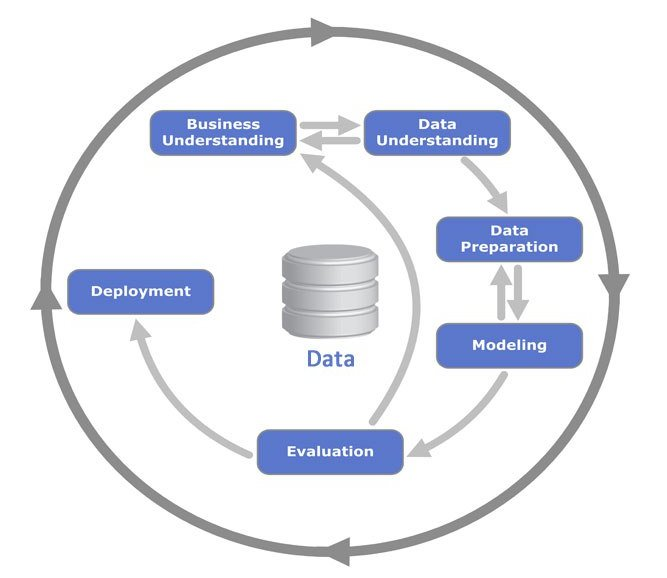
\includegraphics[keepaspectratio=true,scale=0.3]{figuras/crispdmProcess}
	\caption[Modelo de processo CRISP-DM]{Modelo de processo CRISP-DM. Fonte: \citeauthor{CHAPMAN2000} \citeyear{CHAPMAN2000}. p. 10}
	\label{fig:crispdmProcess}
\end{figure}

\begin{itemize}
	\item \textbf{Entendimento do negócio}: atividade inicial que envolve o entendimento dos requisitos da organização, provendo insumos para definir quais dados serão extraídos \cite{CHAPMAN2000}. 
    \item \textbf{Entendimento dos dados}: explorar os dados almejando identificar suas características, problemas e possíveis informações ocultas \cite{CHAPMAN2000}.
    \item \textbf{Implantação}: a implantação é a ação de propor valor para a empresa ou para o consumidor através dos resultados obtidos do processo. Inclui também a entrega do modelo treinado \cite{CHAPMAN2000}.
\end{itemize}

A seguir será apresentada as atividades de um fluxo de trabalho para projetos de \textit{Machine Learning}.

\begin{itemize}
	\item \textbf{Obter dados históricos}: coletar dados históricos sobre o problema a ser resolvido, extrair as características dos dados e organizá-los estruturadamente, identificando dados faltantes, realizar um pre-processamento. Basicamente, executar as atividades da engenharia de características, na qual é o conjunto de técnicas e ferramentas para transformação dos dados em um projeto de ML \cite{BRINK2015}.
    \item \textbf{Construir um modelo}: construir ou utilizar um modelo que seja capaz de lidar bem com a natureza dos dados explorados na atividade de "Obter dados históricos" e que atenda aos objetivos do projeto. Ou seja, em problemas de classificação, o modelo deve classificar corretamente os rótulos de novas amostras \cite{BRINK2015}.
    \item \textbf{Utilizar modelo}: com os dados resultantes da obtenção dos dados e da construção do modelo, faz-se uso do modelo para novos dados e obter as respostas
    \item \textbf{Validar modelo}: os modelos utilizados precisam passar pelo teste de lidar com novos dados. Através dos resultados obtidos destes testes deve-se utilizar métricas adequadas a cada tipo de problema para identificar se o modelo teve bom resultado \cite{BRINK2015}.
    \item \textbf{Otimizar o modelo}: após coletar o resultado das métricas, cabe ao desenvolvedor de um projeto de ML ter capacidade crítica, conhecimento do domínio e de técnicas para propor melhorias ao projeto e obter melhores resultados nas métricas. São três principais modos de melhorar: trocando os parâmetros do modelo, selecionando outro conjunto de características e/ou melhorando a engenharia de características \cite{BRINK2015}.
\end{itemize}

\subsection{Processo Final}

Em projetos de \textit{Data Science} que incluem ML, a melhor metodologia para o desenvolvimento é o CRISP-DM \cite{CROWSTON2017}.
Portanto, será utilizada uma junção das atividades de um projeto de pesquisa com as de projeto de ML.

\begin{figure}[h]
	\centering
    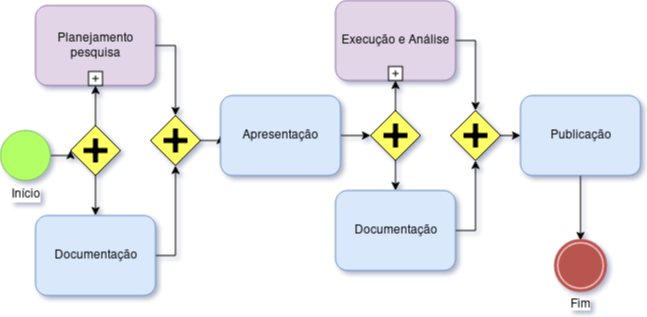
\includegraphics[keepaspectratio=true,scale=0.5]{figuras/processoPrincipal}
	\caption[Processo desenvolvimento da pesquisa]{Processo desenvolvimento da pesquisa. Fonte: elaboração própria}
	\label{fig:processoPrincipal}
\end{figure}

A Figura \ref{fig:processoPrincipal} trás a visão geral de como serão desenvolvidas as atividades do projeto. A atividade de Documentação será executada em paralelo durante todo o projeto, exceto nas etapas de apresentação e publicação.

Das atividades da seção \ref{sec:projetoPesquisa}, temos que as de "Coletar dados", "Tabular e apresentar os dados", "Analisar e interpretar os dados" foram substituídas pelo fluxo de atividades de um projeto de ML. Esta substituição deve-se pela natureza do problema a ser resolvido, pois exige um fluxo diferenciado para análise dos resultados e obtenção dos dados, as quais já foram definidas num projeto de ML descrito na seção \ref{sec:projetoML}.

\begin{figure}[h]
	\centering
    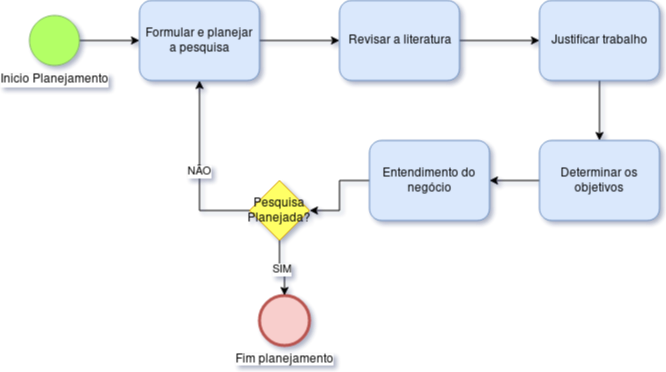
\includegraphics[keepaspectratio=true,scale=0.5]{figuras/subprocessoPlanejamento}
	\caption[Subprocesso planejamento da pesquisa]{Subprocesso planejamento da pesquisa. Fonte: elaboração própria}
	\label{fig:subprocessoPlanejamento}
\end{figure}

Além disso, na \ref{fig:subprocessoPlanejamento}, foi adicionada a atividade "Entendimento do negócio" para melhorar a compreensão do problema do ponto de vista de um trabalho de ML, o que facilitará inclusive o desenvolvimento da pesquisa \cite{CROWSTON2017}.

\begin{figure}[h]
	\centering
    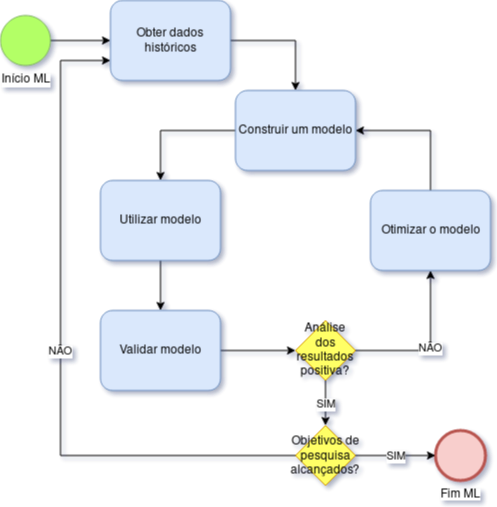
\includegraphics[keepaspectratio=true,scale=0.5]{figuras/subprocessoAnalise}
	\caption[Subprocesso execução e análise]{Subprocesso execução e análise. Fonte: elaboração própria}
	\label{fig:subprocessoAnalise}
\end{figure}

Na Figura \ref{fig:subprocessoAnalise}, foi definido o fluxo de ML semelhante ao proposto por \citeauthor{BRINK2015} (\citeyear{BRINK2015}). A única diferença, é que para os propósitos de pesquisa, foi adicionado mais uma condição que é: "Os objetivos da pesquisa foram alcançados?". Esta pergunta guiará o desenvolvimento do projeto para que, mesmo com ótimos resultados no modelo, a pesquisa tenha prosseguimento e seja possível alcançar seus objetivos.

A atividade "Entendimento dos dados" foi removida do fluxo CRISP-DM, visto que há uma outra atividade de "Obtenção dos dados" que possui equivalência. A outra de Implantação, foi removida, pois ela é para projetos de \textit{Data Science} e a atividade equivalente a esta no trabalho científico é a de Publicação dos resultados.

\section{Cronograma}

A seguir será apresentado uma visão macro do cronograma na Tabela \ref{tab:cronograma}.
\begin{table}[h]
	\centering    
	\caption{Planejamento macro de atividade0s. Fonte: elaboração própria.}
    \label{tab:cronograma}
	\begin{tabular}{|l|p{0,4cm}p{0.4cm}|p{0.4cm}p{0.4cm}p{0.4cm}p{0.4cm}|p{0.4cm}p{0.4cm}p{0.4cm}p{0.4cm}p{0.4cm}|p{0.4cm}p{0.4cm}p{0.4cm}p{0.4cm}|}
    	\hline
		& Março & & Abril & & & & Maio & & & & & Junho & & &  \\ \hline
Macro Tarefa                                   & 1 & 2 & 1 & 2 & 3 & 4 & 1 & 2 & 3 & 4 & 5 & 1 & 2 & 3 & 4 \\ \hline
Formular pesquisa                              & X & X & X &   &   &   &   &   &   &   &   &   &   &   &   \\ \hline
Revisar literatura                             &   &   &   & X & X & X &   &   &   &   &   &   &   &   &   \\ \hline
\makecell[l]{Definição de \\ objetivos específicos}             &   &   &   &   &   &   & X &   &   &   &   &   &   &   &   \\ \hline
Levantar necessidade STF                       &   &   &   &   &   &   &   & X &   &   &   &   &   &   &   \\ \hline
Contexto NLP e ML                              &   &   &   &   &   &   &   & X &   &   &   &   &   &   &   \\ \hline
Contextualização ML              &   &   &   &   &   &   &   & X & X &   &   &   &   &   &   \\ \hline
Metodologia                                    &   &   &   &   &   &   &   &   & X & X &   &   &   &   &   \\ \hline
Referencial ML              &   &   &   &   &   &   &   &   &   & X & X &   &   &   &   \\ \hline
\makecell[l]{Referencial de entendimento \\ do negócio} &   &   &   &   &   &   &   &   &   & X & X &   &   &   &   \\ \hline
\makecell[l]{Procedimentos de obtenção\\ de dados}             &   &   &   &   &   &   &   &   &   &   & X & X &   &   &   \\ \hline
Análise exploratória dos dados                 &   &   &   &   &   &   &   &   &   &   &   & X & X &   &   \\ \hline
Finalização do texto      &   &   &   &   &   &   &   &   &   &   &   &   & X &   &   \\ \hline
Defesa                                         &   &   &   &   &   &   &   &   &   &   &   &   &   &   & X \\ \hline
	\end{tabular}
\end{table}